\chapter{Stakeholders}
\label{chapter:stakeholders}
Stakeholders are an essential source of information for answering the research question. In this chapter, the relevant stakeholders are analyzed and the resulting interview plan is given. Then, the interview results are outlined and the stakeholder analysis is updated. 

\section{Stakeholder analysis} \label{par:stakeholderanalysis}
The relevant stakeholders related to dredging practices in the Rio Paraná Guazú were identified. The interests and goals of the stakeholders are explained, and a power versus interest matrix evaluates their relevance to the project.

\subsection{Stakeholders Description, Interest, and Power}
All relevant stakeholders were identified for this project, some suggested by INA staff and others through further investigation. The complete list is in Table \ref{tab:stakeholders} and will be discussed in the following sections. The stakeholder descriptions are in Table \ref{tab:stakeholders-description}, and their interests and goals in Table \ref{tab:stakeholders-interests-goals}.

\subsubsection{Stakeholders}
Investigation of the relevant parties has lead to a list of 8 stakeholders, the list can be seen in table \ref{tab:stakeholders}. Contact was made with all stakeholders to arrange interviews.

\begin{table}[H]
\centering
\begin{tabularx}{\linewidth}{p{3.5cm}X} % narrower first column
\toprule
Stakeholders & Role \\
\midrule
Dredgers & Extraction of sand and gravel from shallow river areas. \\
\midrule
Prefectura Naval Argentina (PNA) & Protection of rivers and maritime territory, and functions as coast guard and river police. \\
\midrule
Agencia Nacional de Puertos y Navegación (ANPYN) & Oversight of signalling systems, dredging operations, and maintenance of the Main Waterway. \\
\midrule
Ports & Handling, storing, and trading of goods and dredged material. \\
\midrule
Fishers & Artisanal and independent fishing activities for local and regional markets. \\
\midrule
NGOs & Non-profit organizations advocating for environmental protection and community interests. \\
\midrule
Landowners & Owners of riverfront or adjacent lands, may lease property for port or dredging operations. \\
\midrule
Filmmakers & Filmmakers documenting trade and social impacts of the Paraná–Paraguay waterway. \\
\bottomrule
\end{tabularx}
\caption{Potential stakeholders and their roles}
\label{tab:stakeholders}
\end{table}

\newpage

\subsubsection{Description}
In table \ref{tab:stakeholders-description} the stakeholders are listed along with a description of who they are.

\begin{table}[H]
\centering
\begin{tabularx}{\linewidth}{p{3.5cm}X} % fixed width first column
\toprule
Stakeholders & Description \\
\midrule
Dredgers & Dredgers extract sand and gravel from the Paraná Guazú, ranging from small independent vessels to organized groups of boats (areneros) and larger hopper ships. They operate mainly in shallow areas where simple extraction methods are possible, transporting the material to nearby ports such as Ibicuy or Brazo Largo. \\
\midrule
Prefectura Naval Argentina (PNA) & Prefectura Naval Argentina (PNA) serves as Argentina’s coast guard and river police, operating under the Ministry of National Security. It is responsible for protecting rivers and maritime territory, ensuring safety, security, and regulatory compliance. In the Paraná Guazú, PNA plays a key role in monitoring dredging activity and maintaining lawful use of waterways. \\
\midrule
Agencia Nacional de Puertos y Navegación (ANPYN) & Agencia Nacional de Puertos y Navegación is the authority in charge of implementing and controlling the signalling system, as well as overseeing dredging and maintenance along the Main Waterway, which includes the Paraná Guazú. As an independent agency within the Ministry of Economics, it ensures navigational safety and operational continuity of ports and waterways. \\
\midrule
Ports & Ports serve as key logistical hubs for handling and storing goods extracted or transported along the Paraná Guazú. They provide the facilities where dredged sand is unloaded and traded, connecting local extraction activities with broader commercial markets. Their role is essential in enabling the flow of materials and supporting both regional trade and industrial supply chains. \\
\midrule
Fishers & Fishers on the Paraná Guazú depend on the river’s abundant fish resources, particularly migratory species such as sábalo, surubí, boga, pacú, and dorado. Most are independent artisanal fishers, selling their catch through middlemen, freezing plants, or informal markets. Although associations exist in the region, they hold little influence in decision-making over river use and management. \\
\midrule
NGOs & Non-governmental organizations play a role in monitoring the social and environmental impacts of activities along the Paraná Guazú. They advocate for sustainable river management, community interests, and the protection of ecosystems affected by dredging and trade. Their involvement adds external oversight and pressure on both companies and authorities to adopt responsible practices. Major players in the region of the Paraná are WWF,   \\
\midrule
Landowners & The landowners in the area have an interest in the sand mining activities. After all, some of them live in the area and they will experience any negative consequences to their land. Jorge Moriatan is a local landowner that was contacted during the study to tell about his experiences related to the dredging. \\
\midrule
Filmmakers & Alejo Di Risio is a filmmaker who directed a documentary on the Paraná–Paraguay waterway, focusing on the impacts of trade along the river system. His work highlights the economic and social dimensions of waterway use, bringing public attention to stakeholders and their activities. He was also contacted during this study to provide additional insights into stakeholders and businesses connected to the waterway. \\
\bottomrule
\end{tabularx}
\caption{Stakeholder descriptions}
\label{tab:stakeholders-description}
\end{table}

\subsubsection{Interests and Goals}
From the interviews that were carried out, the stakeholder's interests and goals were derived. In Appendix \ref{chap:interviews}, the fully typed out interviews can be found.

\begin{table}[H]
\centering
\begin{tabularx}{\linewidth}{p{3.5cm}XX}
\toprule
Stakeholders & Interest & Goal \\
\midrule
Dredgers & Access to shallow river areas for sand extraction. & Sell extracted sand to nearby ports and local markets for income. \\
\midrule
Prefectura Naval Argentina (PNA) & Safety and security of rivers and maritime territory. & Enforce regulations, monitor dredging, and ensure lawful use of waterways. \\
\midrule
Agencia Nacional de Puertos y Navegación (ANPYN) & Oversight of navigation safety and waterway infrastructure. & Implement signalling systems, maintain dredging operations, and secure efficient transport. \\
\midrule
Ports & Handling and trading of goods and dredged material. & Strengthen logistical capacity and support regional trade flows. \\
\midrule
Fishers & Access to fish resources in the Paraná Guazú. & Sustain livelihoods through artisanal fishing and market sales. \\
\midrule
NGOs & Environmental protection and community rights. & Promote sustainable river management and hold stakeholders accountable. \\
\midrule
Landowners & Protection of riverfront property and prevention of erosion, flooding, or land loss. & Safeguard land rights and preserve long-term property value. \\
\midrule
Filmmakers & Research and documentation of waterway dynamics. & Raise awareness through film on trade, impacts, and stakeholder activities. \\
\bottomrule
\end{tabularx}
\caption{Stakeholders interest and goal}
\label{tab:stakeholders-interests-goals}
\end{table}

\subsection{Stakeholder's Influence}
After identifying stakeholders, it is important to evaluate their power and interest in the project. This is visualized using a power versus interest matrix, with power on the vertical axis and interest on the horizontal axis. Analyzing this matrix informs strategies to approach specific stakeholders. In addition to interest and power, a support-opposition matrix is analyzed to visualize the likelihood that a certain stakeholder will support or oppose the project.

\subsubsection{Power vs. Interest}
The power versus interest matrix is divided into four parts, illustrated in Figure \ref{fig:power-interest}. The quadrants represent the power and interest that a particular stakeholder has in terms of low or high. High power and high interest are referred to as the players, and these will be of most importance to the project. Next, the quadrant with low power and high interest is considered the subject. Those with high power but low interest are determined as the context setters. The context setters are not closely related to the project, but can be of great importance. The quadrant of low power and low interest is recognized as the crowd.

\begin{figure}[H]
    \centering
    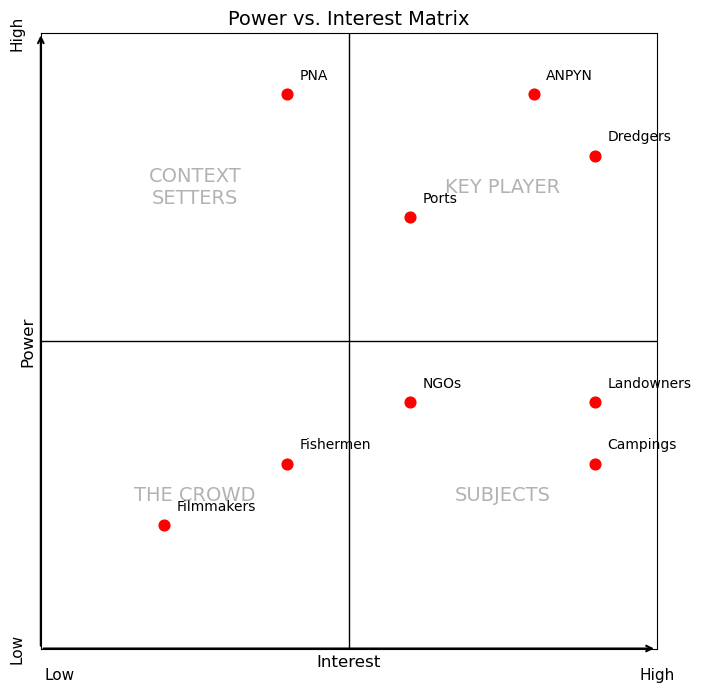
\includegraphics[width=0.70\linewidth]{figures/ch3/PowerVSInterest.png}
    \caption{Power vs. Interest}
    \label{fig:power-interest}
\end{figure}

The key players, stakeholders with both high interest and power, are of great importance to the project. Among this group, there are the actors with a great economic interest in the dredging activity: the dredgers and the ports. They are commercially organized, which is why their power is also high. Finally, the ANPYN, being the responsible government agency, is an actor with both a great interest and power.

This is the most important group for project success. These stakeholders must be actively engaged and managed through continuous and tailored communication. They should be consulted in decision-making and kept up to date on risks, challenges, and progress. Building strong relationships with them is vital to ensure their ongoing support and alignment with project goals.

Context setters have high power but relatively low interest in the project. Within this group, the PNA can be found. Being a major government organization responsible for safety and compliance with maritime laws, they have significant authority and influence. However, their focus will most likely not be on the Paraná Guazú.

The context setters are of moderate priority to the project. Since they hold power, it is important to prevent dissatisfaction that could derail progress. The dealing strategy should focus on maintaining their satisfaction without overwhelming them with details. Periodic check-ins and concise reports or briefings can help with this. This ensures they feel respected and considered, as their influence may become critical if project circumstances shift.

On the bottom right of the graph, one can find the subjects, a group that holds high interest in the project but has less power. Here the NGOs, landowners and campings can be found. Because of ideological believes or personal concerns, their interest in the project is high. However, due to a limited degree of organization their power is not substantial.

This is another group of moderate priority to the project. The stakeholders care deeply about the project but lack significant power to influence its direction. Any enthusiasm from this group can be valuable and should thus be maintained and leveraged if useful. However, it is perhaps more likely for stakeholders in the group of subjects to be opposed to the project. In this case, their high level of interest may manifest as opposition or criticism. Therefore, it is important to listen actively to their concerns and provide information to address any misconceptions or fears. This way, any opposition can be managed and maintained.

Finally, there is the crowd. Stakeholders in this group are characterized by a low power and low interest in the project. The journalists and fishers fall under this group: they are largely unorganized and, although sometimes important, sand mining is not their main concern.

This group is the least important to the project's outcomes. Since their involvement is not crucial, one should avoid overloading them with unnecessary details and should instead only monitor them. It is possible to update the crowd on important progress as to prevent disengagement or frustration.

\subsubsection{Power vs. Support-Opposition}
The support-opposition matrix is divided into four parts and a linear trend line is based on the points given to the stakeholders. On the vertical axis, the division between support and opposition is made, while on the horizontal axis, the power is represented. For the degree of power, the power versus interest matrix, in Figure \ref{fig:power-interest} was used. The stakeholders support or opposition for the project was based on the interviews held during the field trip and is shown in Figure \ref{fig:support-opposition-power}.

\begin{figure}[H]
    \centering
    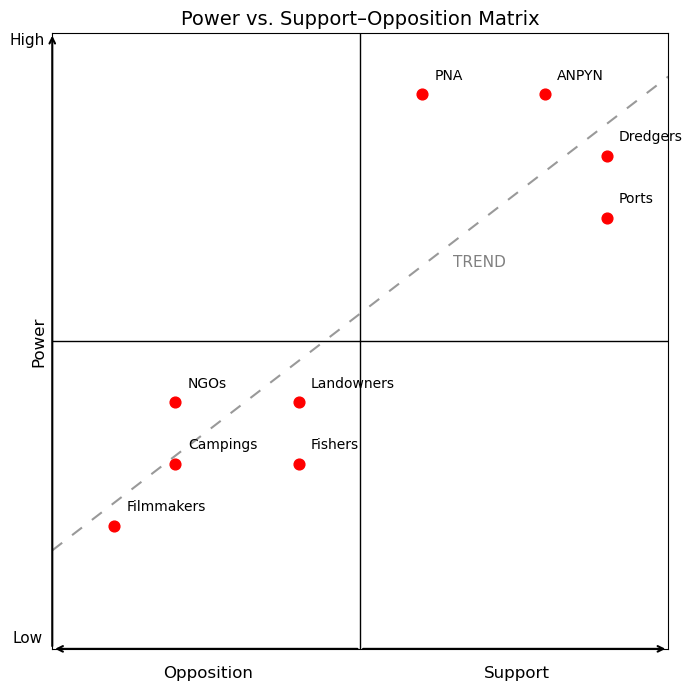
\includegraphics[width=0.70\linewidth]{figures/ch3/Support-OppositionVSPower.png}
    \caption{Power vs. Opposition-Support}
    \label{fig:support-opposition-power}
\end{figure}

\newpage

\subsubsection{Competing Interests}

With different stakeholders who have other interests and goals, it is of importance to know the competing interests. From the different interests of the stakeholders, the competing interests which will be looked into are regarding economic and environmental.

The first competing interest is the economic growth of the area versus environmental protection. The dredging activities of the Parana Guazú and Ibicuy stimulate the economic growth of the area and are one of the income streams for the dredgers and ports. These economic benefits are prioritized over the environmental protection of the river and the river banks. Environmental protection is of interest to fishermen and NGOs that are operating in the Parana waterway. Their goal is to minimize the environmental impact of dredging. This leads to a competing interest, as dredging will have effects that come at the expense of the environment.

A second competing interest is the safety and regulations versus the profits made by the dredging activities. For the business-related stakeholders, the interest in making profits is of higher value than the safety regulations created by the governmental organizations. The PNA and ANPYN regulate the safety of waterways, which can impose restrictions on the amount of sand a dredger can extract or the frequency limit for dredging activities. This can be a concern, as the regulations will cut profits of ports and dredgers, which lie between the strict enforcement and the loosely regulated operations of dredgers.

Another area of conflicting interests can be summarized by local livelihood versus local development. The dredging of the river will lead to income for the ports and dredgers, which, through taxes, can attribute to development of the region in the long run. This can be of interest to local businesses and communities. On the other hand, there is the local livelihood that may be of even greater importance to the community. As mentioned before in chapter \ref{chapter:background}, dredging can reduce water quality, fish spawning and land loss, among other things. A reduction of fish in the river will harm food security in the region and is even more problematic for the fishers, since this directly hurts their businesses and livelihood. Likewise, land loss through increased erosion negatively affects landowners, reducing both property value and security.

Finally, a fourth conflict was identified that deals with property rights on the one hand and public river use on the other. Some stakeholders, such as landowners and ports, have an interest in protecting their private landholdings near the dredging site. After all, protecting their property is of economic interest to them. Some other actors, however, have a greater interest in maintaining open access to the waterways and shorelines. This is for instance the case for the fishers: access to the river and its sides is of crucial importance to their businesses. NGOs are likely to stand on this part of the conflict too since public use of the river and its resources is tied to community rights and local well-being.

% \section{Dredgers (LOCAL??)}
% The first dominant group of stakeholders are the dredgers.These include the local boats used in the area to extract sand and gravel from the river. There are several different types of dredgers ranging from small independent boats, to groups of small boats that work for the same employer (ARENEROS??), or big extracting ships commonly referred to as 'hoppers'. In the area of interest, the Paraná Guazú from Ibicuy to Brazo Largo, the most common dredgers are: (ARENEROS, INDEPENDENT BOATS). 

% Currently there are 2 active boats in the zone of the Rio Paraná Guazú of interest, and (QUITE A LOT MORE IN IBICUY?? FROM INTERVIEW), as mentioned in the previous Chapter. (DREDGING ACTIVITY AANGEVEN WELKE BOTEN, MAPS MET HEEN EN TERUG REIS, DATA , ETC)

% Their interest in the Rio Paraná Guazú is to extract the sand in locations of the river that are shallow since they do not possess any technology to mine the sand from deep. Once this water mixed sand is lifted onto the boat, they transport it to the nearest ports, Ibicuy or Brazo Largo. They sell their sand to the highest bidder which can be for (PURPOSES FROM INTERVIEW).


% \section{BIG Dredging Companies?}
% because they buy the sand and employ the areneros?
% The Dredging companies active in the Rio Paraná Guazú are :
% (EERST KIJKEN OF YPF, JAn de NUl, etc hierbij kan worden betrokken of niet)


% \section{Prefectura Naval Argentina}
% The Prefectura Naval Argentina (PNA), is the National Naval Prefecture of the Rio Paraná. Therefore, they are also active in the Paraná Guazú and our area of surveillance. 
% It is in their interest to protect the Rio Paraná Guazú from criminal activities. These can 

% \section{Agencia Nacional de Puertos y Navegación}
% The Agencia Nacional de Puertos y Navegación (ANPYN), or the National Agency of Ports and Navigation, was created on January 6, 2025 by a merger of the Undersecretariat of Ports, Waterways and Merchant Marine and the General Port Administration. Since then, the agency has taken over the tasks of the two former entities and is now responsible for policies concerning ports, waterways and river and maritime transport. As such, keeping the Vía Navegable Troncal (VNT), Argentina's main waterway, navigable for ships is an important task for the agency. To achieve this, they regulate dredging and sand mining contracts and oversee compliance with the relevant regulations \autocite{boletinoficialdelarepublicaargentinaAgenciaNacionalPuertos2025}.

% \section{Ports}
% In the researched area there are two strategic port locations that play a key role in the sand extraction.

% \subsection{Guazú}
% ?
% \subsection{Ibicuy}
% ?

% \section{fishers}
% Fischermen is another stakeholder group relevant for this study. The Rio Paraná Guazu is used by a lot of people for its high concentration of fish. 

% The artisanal fisheries play an economic role as most of the harvest is sold to middlemen, freezing plants, or in informal markets. Of particular interest are long-range migratory species such as sábalo (Prochilodus lineatus), surubí (Pseudoplatystom corruscans, P. reticulatus), boga (Megaleporinus obtusidens), pacú (Piaractus mesopotamicus), and dorado (Salminus brasiliensis), that support artisanal, recreational, and subsistence fisheries, as observed in other large neotropical rivers, \autocite{assessment of sabalo}, \autocite{fishers' knowledge}

% the fischermen in the region of interest are mostly independent. Even though there exists such thing as fischermen associations in the Rio Paraná Guazú, they are not influencial 



% \section{NGO's}
% even wachten tot ik een nice milieu organisatie vind.

% \section{Agua y Saneamientos Argentinos}
% Even wachten tot interview met hun, kijken of ze wel relevant zijn


% \section{Filmmaker}

% When researching for the stakeholders which were relevant for the analysis. We stumble upon an article on a film that was made on the Parana-Paraguay waterway. In this documentary, the focus is on the impact of the trade happening on the Parana-Paraguay waterway. The documentary is made by filmmaker Alejo Di Risio, who was contacted through journalist Matias Avramow for any additional information about stakeholders and business related to the waterway.

\section{Interview results}
%Wie gesproken, wanneer, hoe benaderd, taal, wie geen reactie

During fieldwork, ten interviews were conducted with the stakeholders listed in Table \ref{tab:stakeholders_results_interviews}. The responses were recorded and these raw results are given in Appendix X. Here, the responses are grouped by theme.

\begin{table}[H]
    \centering
    \renewcommand{\arraystretch}{1.2}
    \setlength{\tabcolsep}{4pt}
    \begin{tabularx}{\textwidth}{l l X c}
        \toprule
        Date & Occupation & Location & Language \\
        \midrule
        24-09-2025 & Caretaker at Fisher's club & 6RJF+C7, Ibicuy, Entre Ríos & Spanish \\
        24-09-2025 & Port manager at Puerto Ibicuy & 6RRC+VC, Ibicuy, Entre Ríos & Spanish \\
        24-09-2025 & Mayor of Ibicuy & 7R5R+4G Puerto Ibicuy, Entre Ríos & Spanish \\
        24-09-2025 & Landowner (Jorge) & 7R5R+4G Puerto Ibicuy, Entre Ríos and his private land & Spanish \\
        25-09-2025 & Municipality Zarate & GLO, Av. Rivadavia 751, B2800GLO Zárate, Provincia de Buenos Aires & Spanish \\
        25-09-2025 & Dredger & Caminera a Ibicuy, Entre Ríos & Spanish \\
        25-09-2025 & Camping owner & Ruta 45 Km 5, E2823, Entre Ríos & Spanish \\
        26-09-2025 & Plant manager YPF & 7XPC+72 Parnacito, Entre Ríos & English \\
        26-09-2025 & Municipality of Zarate & Leandro M. Alem 780, Zárate & Spanish \\
        \bottomrule
    \end{tabularx}
    \caption{Stakeholder overview}
    \label{tab:stakeholders_results_interviews}
\end{table}

\subsection{Dredging activities}
\label{subsec:dredging activities interviews}
The nature of the dredging activities was discussed in nearly all interviews. Different perspectives came forward.
\subsubsection{Number of boats}
Stakeholders provided many insights on the scale and development of dredging in the Paraná Guazú river. The caretaker at the Fisher’s Club didn't perceive any increase in recent years, while nearby landowners recalled that the number of dredgers used to be higher, with only two remaining active today. The mayor of Ibicuy confirmed this trend, explaining that most dredging vessels left the Paraná Ibicuy after municipal taxes on sand extraction were raised. At the Port of Ibicuy, the administrator remembered that small dredgers, no longer than twenty meters, once handled sand but have since disappeared; dredging activities there have ceased altogether and moved to a different port (Port Constanza). A private dredger entrepreneur described his own ship, the Vizcaíno 978, which has been prepared for operation after years of administrative delay.

\subsubsection{Purpose of dredged sand}
Stakeholders also offered insights into the purposes for which dredged sand is used. According to the the mayor, river sand is generally used for construction materials and, in some cases, glass production. The port administrator confirmed that the sand once handled in Ibicuy was also directed toward the construction sector. The dredger entrepreneur described a mixed market, with sand used primarily for concrete, but also increasingly sold to the fracking industry when sufficiently fine-grained. The YPF mine manager confirmed that the company uses river sand for fracking purposes, although not necessarily from the area of interest.

Overall, stakeholders agreed that construction is the traditional destination of dredged sand. However, multiple stakeholders noted that demand for construction sand has declined in recent years, due to the slowdown of public building projects. In contrast, the demand for fracking sand has been growing steadily, as highlighted by the YPF manager. The dredger indicated that selling to YPF might be a viable option.

\subsection{Effects of dredging}
Stakeholders expressed contrasting views on the ecological and geomorphological impacts of dredging in the Paraná Guazú. Mostly the impacts on fish populations and bank stability were discussed.

\subsubsection{Fish populations}
The caretaker of the Fisher’s Club reported a noticeable decline in fish populations. He did not link this directly to the dredging activities, but instead pointed to contamination from agricultural fertilizers. In contrast, a municipal representative from Zárate questioned the narrative of decline, arguing that complaints about fewer fish reflect generational shifts among fishers rather than an actual reduction.

\subsubsection{Riverbank stability}
When it comes to riverbank stability, landowners described severe erosion of up to thirty metres per year, which they attributed to the activities of dredging vessels and passing cargo ships. The caretaker added that vegetation removal near the club increased local erosion. In contrast to this, the mayor of Ibicuy downplayed the role of dredging, attributing bank collapses in his jurisdiction to the natural flow of the river. Futher, in 2011 there was a qual wall collapse in the Port of Ibicuy, but the portmanager claimed that this was an accident and not due to the sand extraction activities.

\subsection{Dry sand mining}
The significance of dry sand mining activities emerged from stakeholder interviews and field observations. Therefore, the topic naturally came up in almost all interviews.
\subsubsection{Extent}
Stakeholders consistently underlined the large scale and rapid growth of dry sand mining in the region. The caretaker at the Fisher’s Club estimated that around 500 trucks leave the area each month carrying 40–45 tons of sand each, noting that this number has doubled compared to when he started his job 4.5 years ago. The mayor of Ibicuy described an even larger scale, reporting that approximately 350 trucks transport some 9,000 tons of sand daily. These impressions were confirmed by the YPF plant manager, who stated that his mine alone extracts about 120,000 tons of sand per month and that output is expected to increase in the coming years. He also referred to geological surveys indicating sufficient reserves to sustain regional extraction for 88 years. This number was confirmed by the mayor, who added that in areas of intense extraction this would be around 40 years.

\subsubsection{Effects}
Multiple effects of these activities were named by interviewees. The caretaker observed that waste from washing processes flows back into the river, making the water dirtier, while the removal of sand on land reduces drainage capacity and therefore increases flooding risks. He and the mayor both emphasized the damage caused by heavy truck traffic, which worsens road conditions and leads to complaints from locals. The mayor added that judicial interventions have forced authorities to introduce extraction limits and monitoring mechanisms, as uncontrolled mining had raised public concerns.

\subsubsection{Purpose}
Stakeholders emphasized that the dominant purpose of dry sand mining in the region is to supply the fracking industry. Both the mayor, port administrator, dredger and the Fisher's club caretaker indicated that most or all dry sand is sold to YPF.

The YPF plant manager explained that the sand extracted is transported primarily to Añelo, in the province of Neuquén, where it is used in fracking operations. He highlighted that this sand is very rich in quarts, is fine-grained and highly resistant, which makes it well-suited for use as proppant, to keep fractures in the shale open during extraction. According to him, these properties are not easily substituted by sand from different locations or other alternatives.

Some stakeholders recalled that also the dry sand was traditionally associated with construction or in some cases glass production, but they acknowledged that these markets have become secondary to the fracking. Part of this is the decreasing demand for construction sand. The port administrator, the YPF mine manager and the dredger all indicated that demand from construction has declined due to the reduction of public building projects. The demand for sand to be used in fracking, on the other hand, is constant according to the dredger and is even increasing according to the YPF manager.

\section{Updated stakeholder analysis}
In paragraph \ref{par:stakeholderanalysis}, an overview of stakeholders was given and each stakeholder's power, interest and support was determined to create a power vs. interest matrix and power vs. support-opposition matrix. Following the stakeholder interviews, some updates to these matrices were necessary.

First of all, in paragraph \ref{par:stakeholderanalysis}, the municipalities were not named as a stakeholder. The assumption was made that ANPYN, the institution responsible for keeping the Main Waterway navigable, was the only government organization with interest in the dredging manners. After an interview with the mayor of Ibicuy, it has become clear that this is in fact not true. Municipalities have an interest in the dredging activities and are therefore included in the updated matrices.

The interest of the municipality is to prevent hindrance to its civilians and to allow for access to the river and therefore their goal is to balance technical river maintenance (via dredging) with the well-being and daily life of civilians and people in the region.

\subsection{Power vs. interest}
In Figure \ref{fig:power-interestNEW}, the updated power versus interest-matrix is shown. After interviewing the port administrator, it became clear that most ports in the area don't handle sand anymore. Therefore, their interest and power has decreased as compared to the first assessment. Secondly, the dredger's power was also reduced, as the dredger explained in the interview that the permit procedure was more difficult than expected. Therefore, their power should be reduced compared to the more powerful government organizations.

On the other hand, the mayor shared insights on how tourist's complaints about dredging vessels caused the municipality to raise taxes on the activity. This caused dredging to stop fully in the Ibicuy area, a clear sign that the power of the tourism industry, i.e. the campings, is greater than what was portrayed in chapter \ref{chapter:stakeholders}. Finally, the power and interest of the municipality are the same as that of the ANPYN.

\begin{figure}[H]
    \centering
    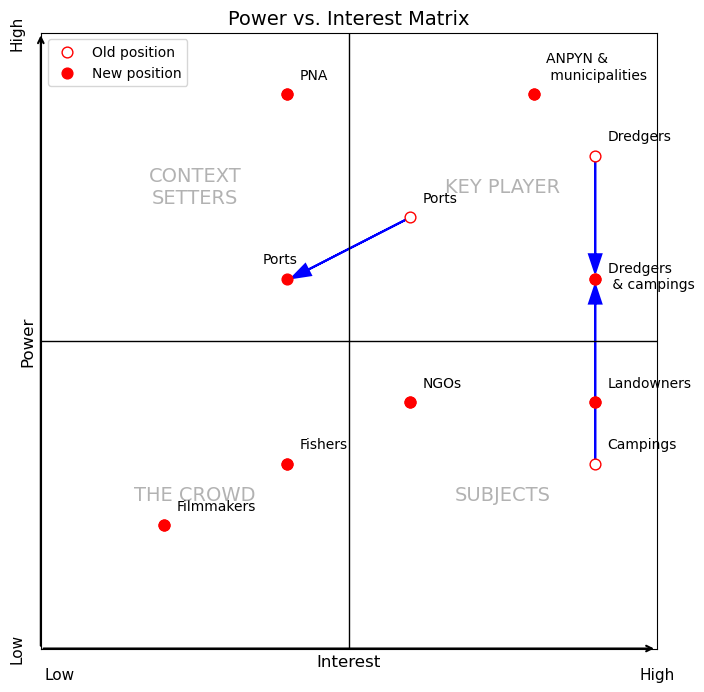
\includegraphics[width=0.70\linewidth]{figures/ch3/NewPowerVSInterest.png}
    \caption{Updated Power vs. Interest}
    \label{fig:power-interestNEW}
\end{figure}

\subsection{Power vs. Support-Opposition}
In figure \ref{fig:power-supportNEW}, the updated power vs. opposition-support-matrix can be found. The powers are updated in the same way as in figure \ref{fig:power-interestNEW} and the degree of opposition was changed for the landowners and campings. From the interviews, many concerns about the dredging operations arose, such as sound pollution and erosion. Many voiced their opposition to the dredging clearly, which is why these stakeholders were moved to the left on the opposition/support scale. For the dredgers and ports, the same degree of support still holds, for monetary reasons. The municipality is opposed to the dredging, as can be seen from the mayor's statements on the discontinuation of dredging.

\begin{figure}[H]
    \centering
    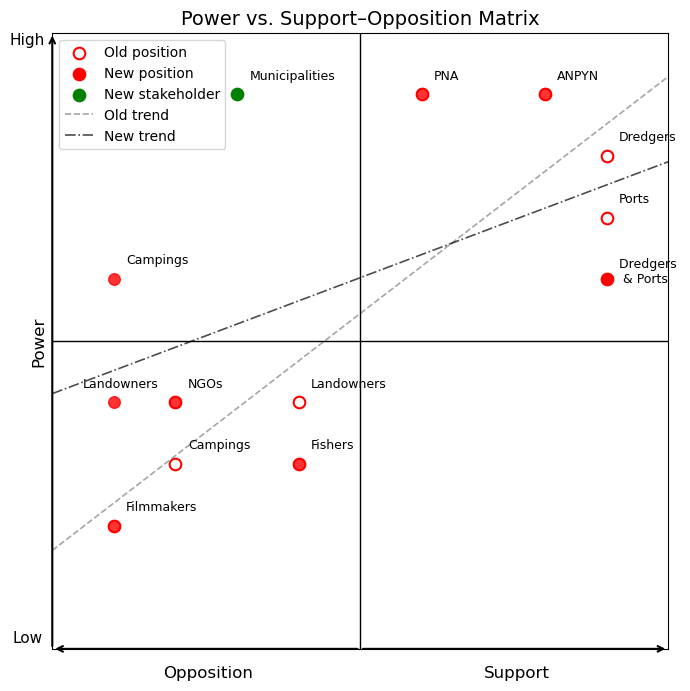
\includegraphics[width=0.70\linewidth]{figures/ch3/NewPowerVSSupport.png}
    \caption{Updated Power vs. Opposition-Support}
    \label{fig:power-supportNEW}
\end{figure}

In Figure \ref{fig:power-supportNEW}, it can be seen that the new trend is flatter than the original one. This is a consequence of the fact that dredging operations have not increased in recent years, as opposed to the expectation, and have in fact been completely stopped on the Paraná-Ibicuy.